\section{第三章}

\subsection{题目1}

求解线性方程组
\begin{align}
	&4x-y+z=7\\
	&4x-8y+z=-21\\
	&-2x+y+5z=15
\end{align}

\begin{enumerate}
	\item 使用LU分解求此方程组
	\item 分别用Jacobi,Gauss-Seidel方法求解此方程组
\end{enumerate}

\subsubsection{题目1.1}

使用LU分解求此方程组。

\paragraph{LU分解}
~\\
给定一个无行交换的高斯消去法可求解一般线性方程组$AX=B$,则矩阵A可分解为一个下三角矩阵L和一个上三角矩阵U的乘积:
\begin{center}
	$A=LU$ 
\end{center}
而且L的对角线元素为1,U的对角线元素非零。
得到LU矩阵之后,原方程变为:
\begin{center}
	$LUX=B$ 
\end{center}
这时可以先把UX当成新的未知数,即求解
$LX_{new}=B$
得到$X_{new}w$之后,再求解
$UX=X_{new}$
最终得到X.

\paragraph{分解矩阵}
~\\
利用已知求未知。最开始已知L的对角线全是1,所以用L的第一行分别与U的第一列、第二列…第n列相乘,得到U的第一行。然后用L的第二行与U的第一列相乘求得L中第二行的所有元素,然后用L的第二行分别与U的所有列相乘求得U的第二行,然后一直重复这样的步骤,就可以得到分解的LU矩阵。
\paragraph{求解矩阵$X_{new}$}
~\\
用L的第一行乘以$X_{new}$的列,求得$X_{new}$的第一行,然后用L的第二行乘以$X_{new}$的列,求得$X_{new}$的第二行。重复这样的步骤就可以得到$X_{new}$的所有值。
\paragraph{求解矩阵$X$}
~\\
类似$X_{new}$的求法,但是是从U矩阵的最后一行向上分别和X的列相乘。
LU分解的代码和分解之后求解方程组的代码:

设$\mathbf{A} = \left(a_{i,j}\right)_{n \times n}$, 分解为$\mathbf{A} = \mathbf{LU}$的形式, 其中$\mathbf{L}$为对角元为1的下三角矩阵, $\mathbf{U}$为上三角矩阵. 即
$$
\left(
\begin{matrix}
a_{11} & a_{12} & \cdots & a_{1n} \\
a_{21} & a_{22} & \cdots & a_{2n} \\
\vdots & \vdots & \ddots & \vdots \\
a_{n1} & a_{n2} & \cdots & a_{nn} \\
\end{matrix}
\right) =
\left(
\begin{matrix}
1 & 0 & \cdots & 0 \\
l_{21} & 1 & \cdots & 0 \\
\vdots & \vdots & \ddots & \vdots \\
l_{n1} & l_{n2} & \cdots & 1 \\
\end{matrix}
\right) 
\left(
\begin{matrix}
u_{11} & u_{12} & \cdots & u_{1n} \\
0 & u_{22} & \cdots & u_{2n}\\
\vdots & \vdots & \ddots & \vdots \\
0 & 0 & \cdots & u_{nn} \\
\end{matrix}
\right)
$$
按照矩阵乘法规则, 比较系数, 可得
$$
\left\{
\begin{aligned}
u_{1j} &= a_{1j}  &\left(j=1,2,\cdots,n\right) \\
l_{i1} &= \frac{a_{i1}}{u_{11}} &\left(i=2,3,\cdots,n \right)\\
u_{ij} &= a_{ij} - \sum_{k=1}^{i-1}l_{ik}u_{kj} &\left(i=2,\cdots,n,j=i,\cdots,n\right) \\
l_{ij} &= \left(a_{ij} - \sum_{k=1}^{j-1}l_{ik}u_{kj}\right) &\left(j=1,2,\cdots,n,i=j+1,\cdots,n\right)
\end{aligned}
\right.$$

分解之后的矩阵:
$$
\mathbf{L} = 
\left(
\begin{matrix}
1 & 0 & 0 \\
1 &  1 & 0 \\
-0.5 &  -0.0714 & 1
\end{matrix}
\right)
\mathbf{U} = 
\left(
\begin{matrix}
4 & -1 & 1 \\
0 &  -7 & 0 \\
0 &  0 & 5.5
\end{matrix}
\right)
$$
方程的解:
\begin{enumerate}
	\item $x_1 = 2$;
	\item $x_2 = 4$;
	\item $x_3 = 3$;
\end{enumerate}

\paragraph{LU分解代码}
~\\
\begin{minted}{python}
A = np.array([[4, -1, 1], [4, -8, 1], [-2, 1, 5]])
B = np.array([7, -21, 15]).reshape(-1, 1)
\end{minted}
\begin{minted}{python}
def pivot_matrix(A):
    m = A.shape[0]
    I = np.identity(m)
    for j in range(m):
        row = max(range(j, m), key=lambda i: abs(A[i, j]))
        if j != row:
            I[[j, row]] = I[[row, j]]
    return I

def lu_decomposition(A):
    n = A.shape[0]
    L = np.zeros((n, n), dtype=float)
    U = np.zeros((n, n), dtype=float)
    A = np.dot(pivot_matrix(A), A)
    for i in range(n):
        for k in range(i, n):
            s = sum(L[i][j] * U[j][k] for j in range(i))
            U[i][k] = A[i][k] - s
        for k in range(i, n):
            if i == k:
                L[i][i] = 1
            else:
                s = sum(L[k][j] * U[j][i] for j in range(i))
                L[k][i] = (A[k][i] - s) / U[i][i]
    return A, L, U

AB = np.column_stack([A, B])
AB, L, U = lu_decomposition(AB)

UX = backsubL(L, B).reshape(-1, 1)
X = backsubU(U, UX).reshape(-1, 1)
\end{minted}

\subsubsection{题目1.2}

分别用Jacobi,Gauss-Seidel方法求解此方程组。

\subparagraph{推导}
假设方程组
$$\left\{
\begin{aligned}
a_{11}x_1 &+ a_{12}x_2 + \cdots + a_{1n}x_n = b_1 \\ 
a_{21}x_1 &+ a_{22}x_2 + \cdots + a_{2n}x_n = b_2 \\ 
&\vdots \\
a_{n1}x_1 &+ a_{n2}x_2 + \cdots + a_{nn}x_n = b_1 
\end{aligned}
\right.$$
的系数矩阵$\mathbf{A}$非奇异, 不妨设$a_{ii} \neq 0\left(i=1,2,\cdots,n\right)$.将方程组变形为:
$$\left\{
\begin{aligned}
x_1 = \frac{1}{a_{11}}&\left(-a_{12}x_2 -a_{13}x_3 -\cdots - a_{1n}x_n +b_1\right) \\
x_2 = \frac{1}{a_{22}}&\left(-a_{21}x_1 -a_{23}x_3 -\cdots - a_{2n}x_n +b_2\right) \\
&\vdots \\
x_n = \frac{1}{a_{nn}}&\left(-a_{n1}x_1 -a_{n2}x_2 -\cdots - a_{n,n-1}x_{n-1} +b_n\right) 
\end{aligned}
\right.$$
建立迭代公式:
$$\left\{
\begin{aligned}
x_1^{\left(k+1\right)} = \frac{1}{a_{11}}&\left(-a_{12}x_2^{\left(k\right)} -a_{13}x_3^{\left(k\right)} -\cdots - a_{1n}x_n^{\left(k\right)} +b_1\right) \\
x_2^{\left(k+1\right)} = \frac{1}{a_{22}}&\left(-a_{21}x_1^{\left(k\right)} -a_{23}x_3^{\left(k\right)} -\cdots - a_{2n}x_n^{\left(k\right)} +b_2\right) \\
&\vdots \\
x_n^{\left(k+1\right)} = \frac{1}{a_{nn}}&\left(-a_{n1}x_1^{\left(k\right)} -a_{n2}x_2^{\left(k\right)} -\cdots - a_{n,n-1}x_{n-1}^{\left(k\right)} +b_n\right) 
\end{aligned}
\right.$$
选定初始向量$\mathbf{x}^{\left(0\right)}$后, 反复迭代可以得到向量序列$\left\{\mathbf{x}^{\left(k\right)} \right\}$
迭代公式为:
$$\left\{
\begin{aligned}
\mathbf{x}^{\left(0\right)} &= \left(x_1^{\left(0\right)},x_2^{\left(0\right),\cdots,x_n^{\left(0\right)}}\right)^T \\
x_i^{\left(k+1\right)} &= \frac{1}{a_{ii}}\left(b_i - \sum_{j=1,j\neq i}^{n}a_{ij}x_j^{\left(k\right)} \right)
\end{aligned}
\right.$$

Jacobi迭代法也可以写为向量递推的形式
$$\mathbf{x}^{\left(k\right)} = \mathbf{T}\mathbf{x}^{\left(k\right)} + \mathbf{c}$$

设$\mathbf{D}$是对角元与$\mathbf{A}$相同的对角阵; $-\mathbf{L}$是严格下三角矩阵, 下三角元素与$\mathbf{A}$相同; $-\mathbf{U}$是严格上三角矩阵, 上三角元素与$\mathbf{A}$相同. 因此$\mathbf{A} = \mathbf{D} - \mathbf{L} - \mathbf{U}$.

对于方程$\mathbf{A} \mathbf{x} = \mathbf{b}$, 或$\left(\mathbf{D} - \mathbf{L} - \mathbf{U} \right) \mathbf{x} = \mathbf{b}$, 

可以变形为$$\mathbf{D} \mathbf{x} = \left(\mathbf{L} + \mathbf{U} \right) \mathbf{x} + \mathbf{b}$$

也就是$$\mathbf{x} = \mathbf{D}^{-1} \left(\mathbf{L} + \mathbf{U}\right) \mathbf{x} + \mathbf{D}^{-1}\mathbf{b}$$

写成递推式的形式: $$\mathbf{x}^{\left(k\right)} = \mathbf{D}^{-1} \left(\mathbf{L} + \mathbf{U}\right) \mathbf{x}^{\left(k-1\right)} + \mathbf{D}^{-1}\mathbf{b}$$

\subparagraph{分析}
由方程组可得:$x=\frac{7+y+z}{4}$,$y=\frac{21+4*x+z}{8}$,$z=\frac{15+2*x-y}{5}$
这样就提出了下列Jacobi迭代过程:

$$ \left\{
\begin{aligned}
x_{k+1} =\frac{7+1*y_k+z_k}{4} \\
y_{k+1} =\frac{21+4 * x_k+z_k}{8} \\
z_{k+1} =\frac{15+2*x_k-y_k}{5}
\end{aligned}
\right.
$$

$\mathbf{x} = \left(2,4,3\right)$, 与求解线性方程组结果一致。

\paragraph{Jacobi迭代的解随迭代次数的变化}

下面对Jacobi迭代的解随迭代次数的变化进行探究,运行Jacobi迭代程序,得到下表。

\begin{table}[H]
	\centering
	\caption{Jacobi迭代的解随迭代次数的变化表}
	\begin{tabular}{llll}
		\hline
		迭代次数 & $x_0$          & $x_1$          & $x_2$          \\ \hline
		0    & 0.000000000000 & 0.000000000000 & 0.000000000000 \\
		1    & 1.750000000000 & 2.625000000000 & 3.000000000000 \\
		2    & 1.656250000000 & 3.875000000000 & 3.175000000000 \\
		3    & 1.925000000000 & 3.850000000000 & 2.887500000000 \\
		4    & 1.990625000000 & 3.948437500000 & 3.000000000000 \\
		5    & 1.987109375000 & 3.995312500000 & 3.006562500000 \\
		6    & 1.997187500000 & 3.994375000000 & 2.995781250000 \\
		7    & 1.999648437500 & 3.998066406250 & 3.000000000000 \\
		8    & 1.999516601563 & 3.999824218750 & 3.000246093750 \\
		9    & 1.999894531250 & 3.999789062500 & 2.999841796875 \\
		10   & 1.999986816406 & 3.999927490234 & 3.000000000000 \\
		11   & 1.999981872559 & 3.999993408203 & 3.000009228516 \\
		12   & 1.999996044922 & 3.999992089844 & 2.999994067383 \\
		13   & 1.999999505615 & 3.999997280884 & 3.000000000000 \\
		14   & 1.999999320221 & 3.999999752808 & 3.000000346069 \\
		15   & 1.999999851685 & 3.999999703369 & 2.999999777527 \\
		16   & 1.999999981461 & 3.999999898033 & 3.000000000000 \\
		17   & 1.999999974508 & 3.999999990730 & 3.000000012978 \\
		18   & 1.999999994438 & 3.999999988876 & 2.999999991657 \\
		19   & 1.999999999305 & 3.999999996176 & 3.000000000000 \\
		20   & 1.999999999044 & 3.999999999652 & 3.000000000487 \\
		21   & 1.999999999791 & 3.999999999583 & 2.999999999687 \\
		22   & 1.999999999974 & 3.999999999857 & 3.000000000000 \\
		23   & 1.999999999964 & 3.999999999987 & 3.000000000018 \\
		24   & 1.999999999992 & 3.999999999984 & 2.999999999988 \\
		25   & 1.999999999999 & 3.999999999995 & 3.000000000000 \\
		26   & 1.999999999999 & 4.000000000000 & 3.000000000001 \\
		27   & 2.000000000000 & 3.999999999999 & 3.000000000000 \\
		28   & 2.000000000000 & 4.000000000000 & 3.000000000000 \\
		29   & 2.000000000000 & 4.000000000000 & 3.000000000000 \\ \hline
	\end{tabular}
\end{table}

\begin{figure}[H]
	\centering
	\caption{Jacobi迭代的解随迭代次数的变化}
	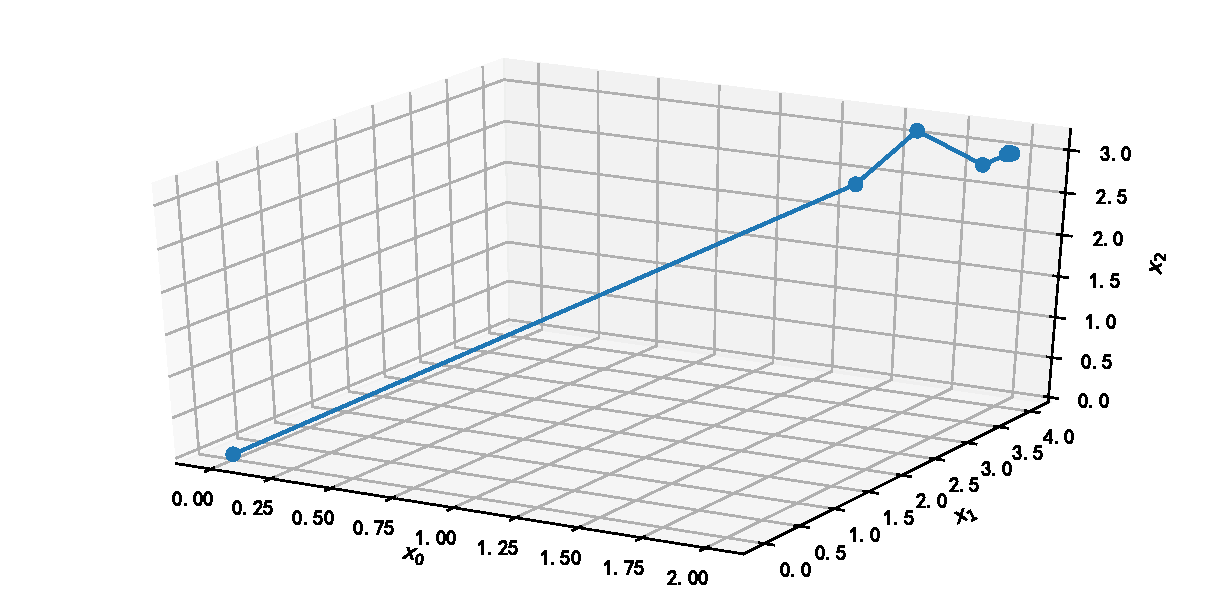
\includegraphics[width=\linewidth]{fig13.pdf}
\end{figure}

\begin{figure}[H]
	\centering
	\caption{Jacobi迭代的每个解随迭代次数的变化}
	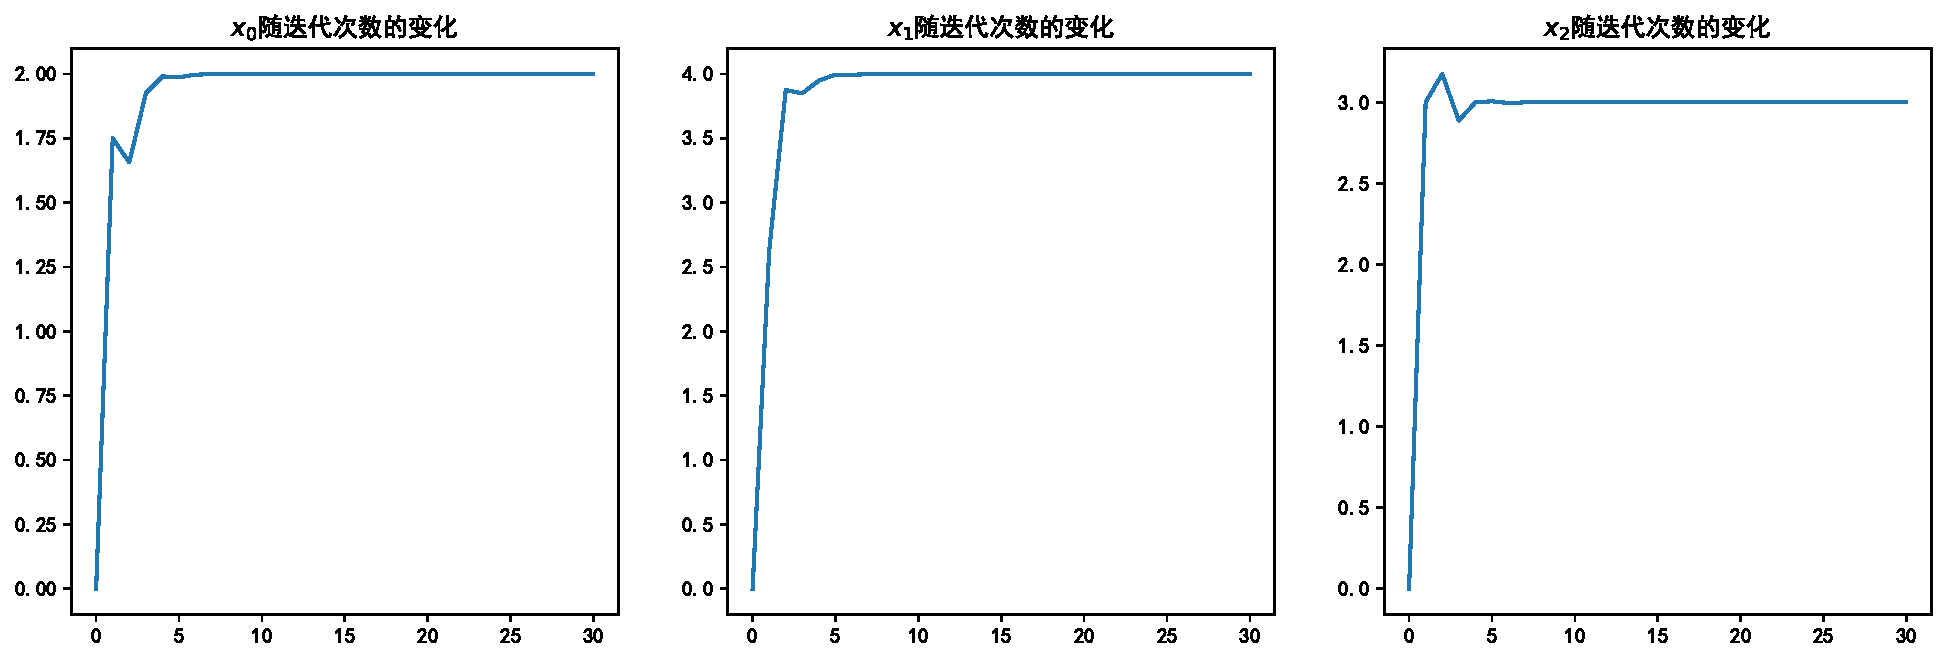
\includegraphics[width=\linewidth]{fig14.pdf}
\end{figure}


\paragraph{Jacobi迭代代码}
~\\
\begin{minted}[mathescape,
               linenos,
               numbersep=5pt,
               frame=lines,
               framesep=2mm]{python}
def jacobi(A, B, max_iter, x=None, ax=None):
    B = B.reshape(-1)
    if x is None:
        x = np.zeros_like(B)
    show = ax is not None and x.size == 3
    showx = [[] for _ in range(3)]
\end{minted}
\begin{minted}{python}
    D = np.diag(A)
    R = A - np.diagflat(D)
    if show:
        for i in range(len(showx)):
            showx[i].append(x[i])
    for _ in range(max_iter):
        x = (B - np.dot(R, x)) / D
        if show:
            for i in range(len(showx)):
                showx[i].append(x[i])
    if show:
        ax.plot(showx[0], showx[1], showx[2], marker='o')
        ax.set_xlabel('$x_0$')
        ax.set_ylabel('$x_1$')
        ax.set_zlabel('$x_2$')
        return x, np.array(showx)
    return x
\end{minted}

\paragraph{Gauss-Seidel方法}
~\\
如果把Jacobi迭代公式改成以下形式
$$\left\{
\begin{aligned}
x_1^{\left(k+1\right)} = \frac{1}{a_{11}}&\left(-a_{12}x_2^{\left(k\right)} -a_{13}x_3^{\left(k\right)} -\cdots - a_{1n}x_n^{\left(k\right)} +b_1\right) \\
x_2^{\left(k+1\right)} = \frac{1}{a_{22}}&\left(-a_{21}x_1^{\left(k+1\right)} -a_{23}x_3^{\left(k\right)} -\cdots - a_{2n}x_n^{\left(k\right)} +b_2\right) \\
&\vdots \\
x_n^{\left(k+1\right)} = \frac{1}{a_{nn}}&\left(-a_{n1}x_1^{\left(k+1\right)} -a_{n2}x_2^{\left(k+1\right)} -\cdots - a_{n,n-1}x_{n-1}^{\left(k+1\right)} +b_n\right) 
\end{aligned}
\right.$$
选取初始向量$\mathbf{x}^{\left(0\right)}$, 用迭代公式:
$$\left\{
\begin{aligned}
\mathbf{x}^{\left(0\right)} &= \left(x_1^{\left(0\right)},x_2^{\left(0\right),\cdots,x_n^{\left(0\right)}}\right)^T \\
x_i^{\left(k+1\right)} &= \frac{1}{a_{ii}}\left(b_i - \sum_{j=1}^{i-1}a_{ij}x_j^{\left(k+1\right)} - \sum_{j=i+1}^{n}a_{ij}x_j^{\left(k\right)} \right)
\end{aligned}
\right.$$
Gauss-Seidel迭代法也可以写为向量递推的形式:
$$\mathbf{x}^{\left(k\right)} = \mathbf{T}_g\mathbf{x}^{\left(k\right)} + \mathbf{c}_g$$
或
$$\left(\mathbf{D} - \mathbf{L}\right) \mathbf{x}^{\left(k\right)} = \mathbf{U} \mathbf{x}^{\left(k-1 \right)} + \mathbf{b}$$
即
$$ \mathbf{x}^{\left(k\right)} = \left(\mathbf{D} - \mathbf{L}\right)^{-1}\mathbf{U}\mathbf{x}^{k-1} + \left(\mathbf{D} - \mathbf{L}\right)^{-1}\mathbf{b}$$

由方程组可得:$x=\frac{7+y+z}{4}$,$y=\frac{21+4*x+z}{8}$,$z=\frac{15+2*x-y}{5}$
这样就提出了下列Gauss-Seidel迭代过程:

$$ \left\{
\begin{aligned}
x_{k+1}& =\frac{7+1*y_k+z_k}{4} \\
y_{k+1}& =\frac{21+4 * x_{k+1}+z_k}{8} \\
z_{k+1}& =\frac{15+2*x_{k+1}-y_{k+1}}{5}
\end{aligned}
\right.
$$

Jacobi方法没有利用刚计算出来的值,而Gauss-Seidel方法利用了刚计算出来的值,Gauss-Seildel方法对于相同的精度应该需要的迭代次数应该比Jacobi方法的要少,即收敛得更快。实际上因为有Stein-Rosenberg定理有:如果对每个$i≠j,a_{ij}≤0$,且对每个$i=1,2,…,n$ $ a_{ii}>0$,那么一下结论有且只有一个成立:

\begin{align*}
0 \leq p(T_g) < p(T_g) < 1\\
1 < p(T_j)<p(T_g)\\
p(T_j)=p(T_g)=0\\
p(T_j)=p(T_g)=1\\
\end{align*}

\paragraph{Gauss-Seidel方法的解随迭代次数的变化}

下面是Gauss-Seidel方法的解随迭代次数的变化表与变化图:

\begin{table}[H]
	\centering
	\caption{Gauss-Seidel方法的解随迭代次数的变化表}
	\begin{tabular}{llll}
		\hline
		迭代次数 & $x_0$          & $x_1$          & $x_2$          \\ \hline
0    & 0.000000000000 & 0.000000000000 & 0.000000000000 \\
1    & 1.750000000000 & 3.500000000000 & 3.000000000000 \\
2    & 1.875000000000 & 3.937500000000 & 2.962500000000 \\
3    & 1.993750000000 & 3.992187500000 & 2.999062500000 \\
4    & 1.998281250000 & 3.999023437500 & 2.999507812500 \\
5    & 1.999878906250 & 3.999877929688 & 2.999975976563 \\
6    & 1.999975488281 & 3.999984741211 & 2.999993247070 \\
7    & 1.999997873535 & 3.999998092651 & 2.999999530884 \\
$\cdots$ & $\cdots$  & $\cdots$  & $\cdots$ \\
24   & 2.000000000000 & 4.000000000000 & 3.000000000000 \\
25   & 2.000000000000 & 4.000000000000 & 3.000000000000 \\
26   & 2.000000000000 & 4.000000000000 & 3.000000000000 \\
27   & 2.000000000000 & 4.000000000000 & 3.000000000000 \\
28   & 2.000000000000 & 4.000000000000 & 3.000000000000 \\
29   & 2.000000000000 & 4.000000000000 & 3.000000000000 \\ \hline
	\end{tabular}
\end{table}

\begin{figure}[H]
	\centering
	\caption{Gauss-Seidel方法的解随迭代次数的变化}
	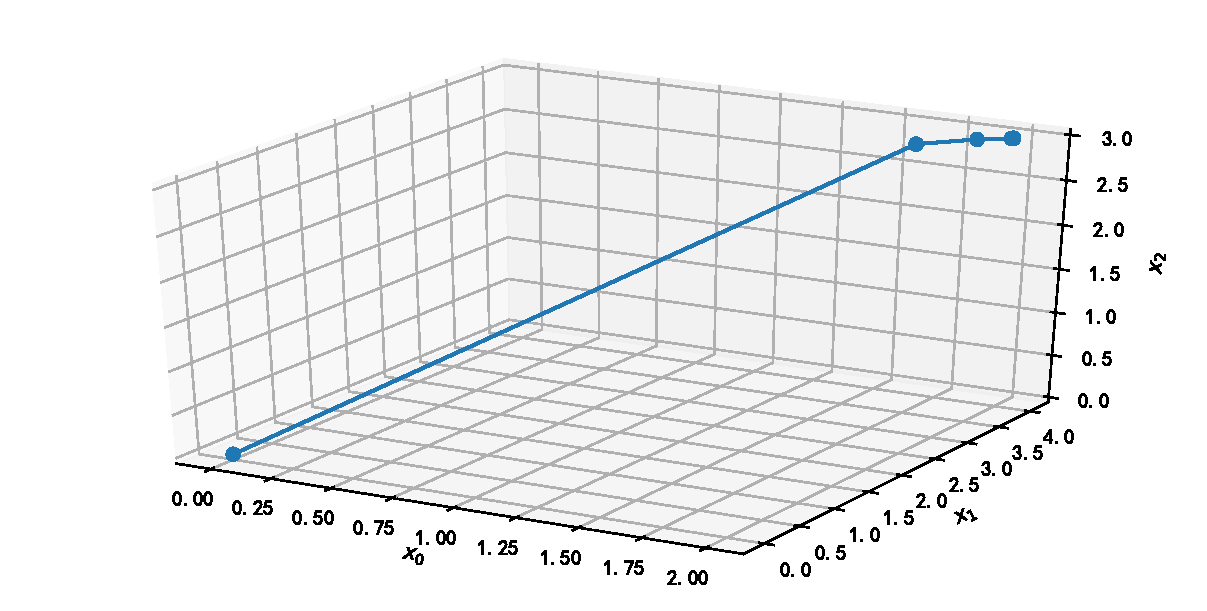
\includegraphics[width=\linewidth]{fig15.pdf}
\end{figure}

\begin{figure}[H]
	\centering
	\caption{Gauss-Seidel方法的每个解随迭代次数的变化}
	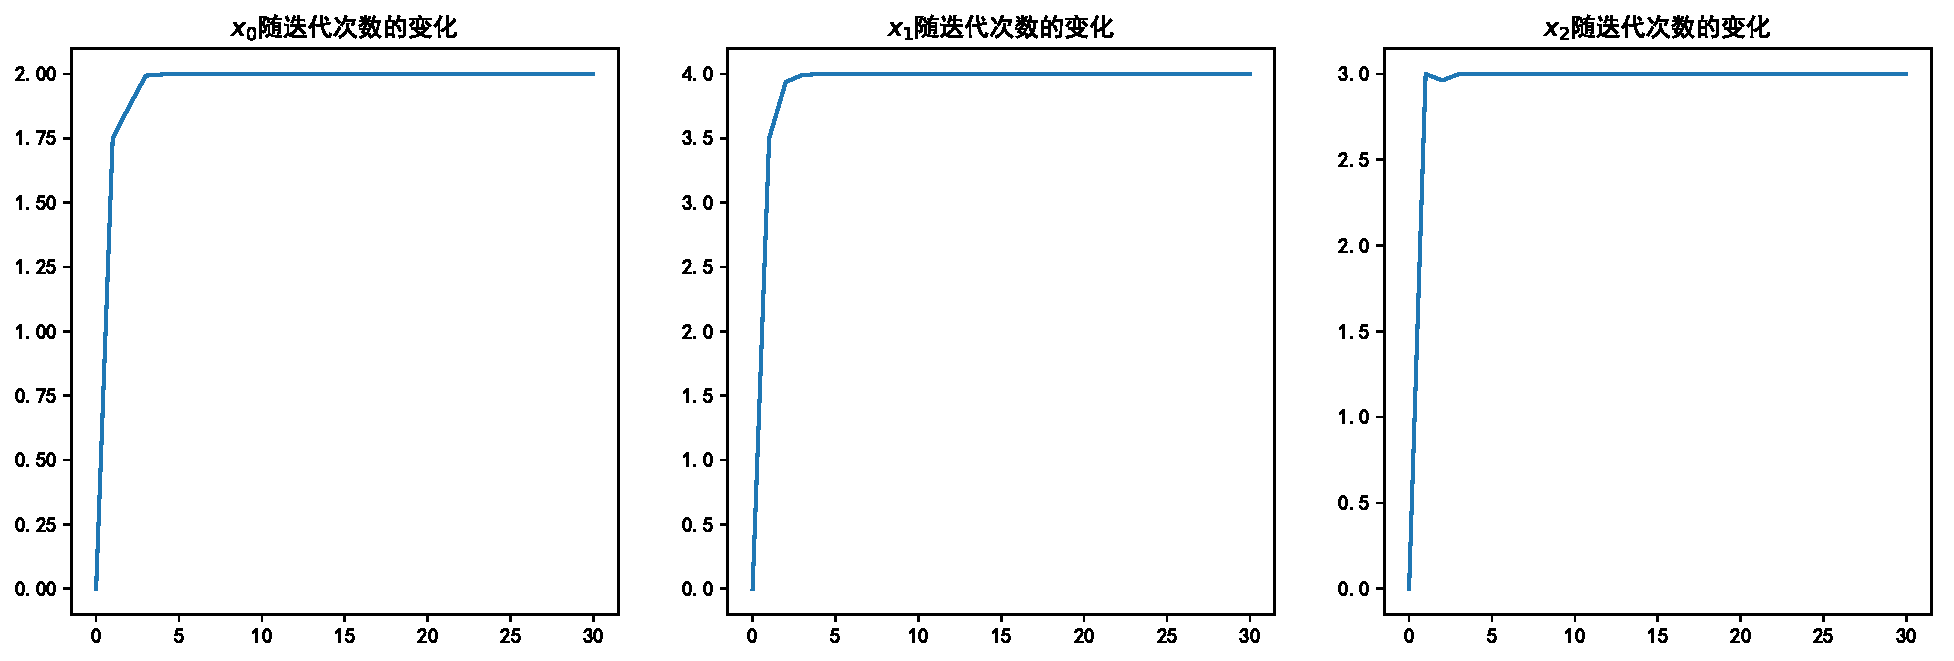
\includegraphics[width=\linewidth]{fig16.pdf}
\end{figure}

\paragraph{Gauss-Seidel方法代码}
~\\
\begin{minted}{python}
def gauss_seidel(A, B, max_iter, x=None, ax=None):
    B = B.reshape(-1)
    if x is None:
        x = np.zeros_like(B)
    show = ax is not None and x.size == 3
    showx = [[] for _ in range(3)]
\end{minted}
\begin{minted}{python}
    if show:
        for i in range(len(showx)):
            showx[i].append(x[i])
    for _ in range(max_iter):
        x_new = np.zeros_like(x)
        for i in range(A.shape[0]):
            s1 = np.dot(A[i, :i], x_new[:i])
            s2 = np.dot(A[i, i + 1:], x[i + 1:])
            x_new[i] = (B[i] - s1 - s2) / A[i, i]
        x = x_new
        if show:
            for i in range(len(showx)):
                showx[i].append(x[i])
    if show:
        ax.plot(showx[0], showx[1], showx[2], marker='o')
        ax.set_xlabel('$x_0$')
        ax.set_ylabel('$x_1$')
        ax.set_zlabel('$x_2$')
        return x, np.array(showx)
    return x
\end{minted}

\paragraph{Jacobi迭代与Gauss-Seidel方法对比}
~\\
下图是Jacobi迭代与Gauss-Seidel方法在每个解上的对比图:

\begin{figure}[H]
	\centering
	\caption{Jacobi迭代与Gauss-Seidel方法对比图}
	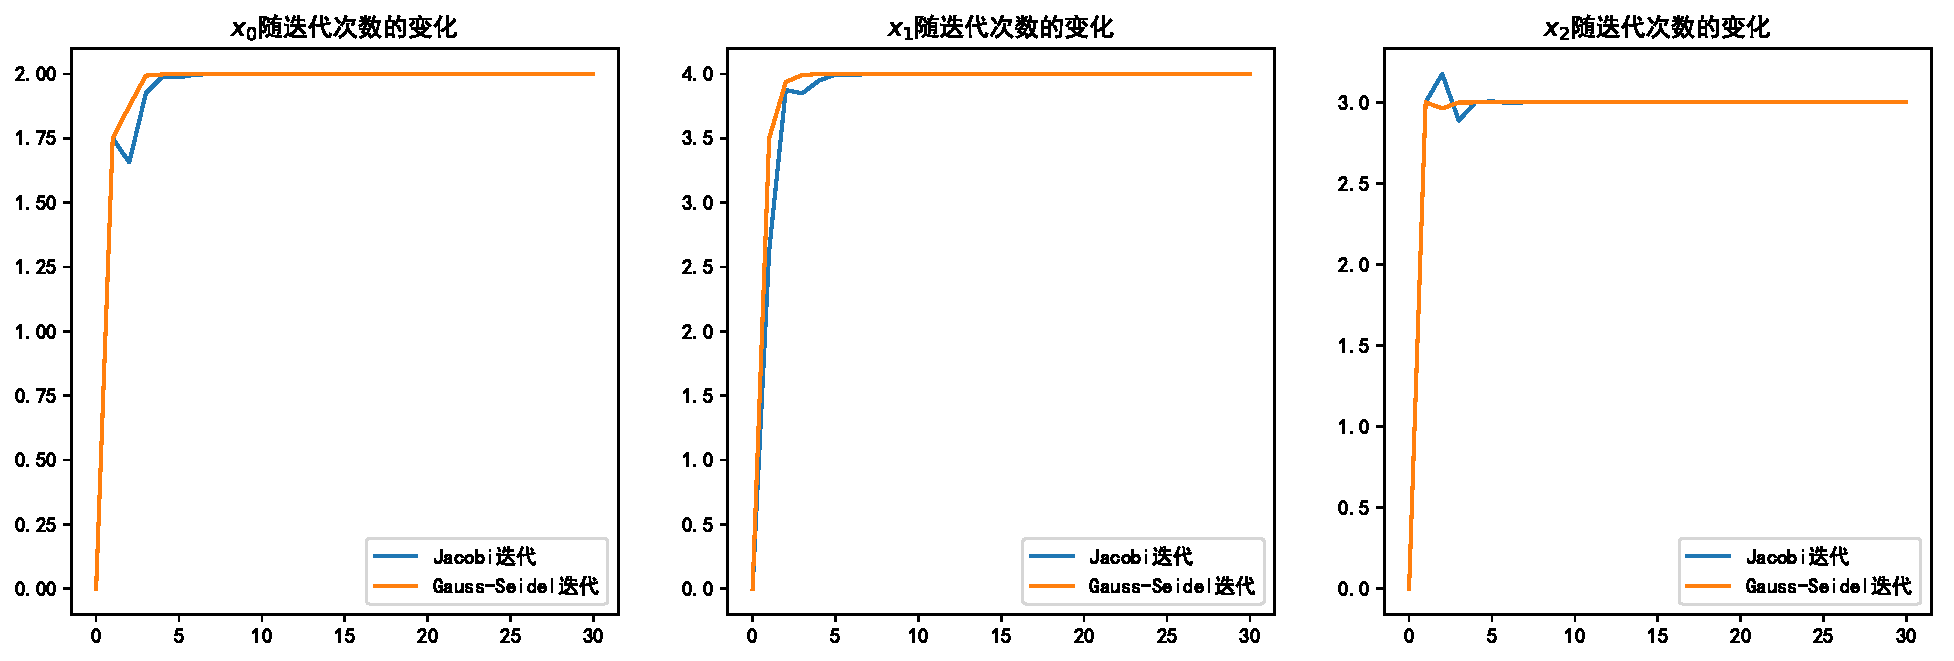
\includegraphics[width=.9\linewidth]{fig17.pdf}
\end{figure}

\subsection{题目2}

设有如下三角线性方程组,而且系数矩阵具有严格对角优势:

$$
\begin{matrix}
d_1x_1 &+&c_1x_2 &  & & & & &=&b_1\\
a_1x_1 &+& d_2x_2&+& c_2x_3 & & & &=&b_2\\
& & a_2x_2 &+& d_3x_3 &+& c_3x_4 & &=&b_3\\
& & . & & & &&&.\\
& &  &. & & &&&.\\
& & & &. & &&&.\\
& & & &  & a_{N-1}x_{N-1}&+&d_Nx_N&=&b_N\\
\end{matrix}
$$

设计一个算法来求解上述方程组. 算法必须有效地利用系数矩阵的稀疏性。

\paragraph{分析}
~\\
对第一行$d_xx_1 +c_1x_2 = b$,将其转变为$x_1 + \frac{c_1}{d_1}x_2 = \frac{b_1}{d_1}$

对将第一行乘$a_1$与第二行相减,把第二行转变为\[(d_2 - \frac{a_1c_1}{d_1})x_2 + c_2x_3 = \frac{c_2}{d_2} - \frac{a_2b_1}{d_1}\]

然后用第二行转化第三行,第三行转化第四行,以此类推。最终矩阵的形式为
\begin{align*}
\begin{pmatrix}
1 & r_1 & &  & \\ 
& 1 & \ddots & & \\ 
&  & 1 & \ddots & \\ 
&  &  & \ddots & r_1\\ 
&  &  &  & 1
\end{pmatrix}
\begin{pmatrix}
x_1\\ 
x_2\\ 
\vdots\\ 
x_{n-1}\\
x_n
\end{pmatrix}
=
\begin{pmatrix}
\rho_1\\ 
\rho_2\\ 
\vdots\\ 
\rho_{n-1}\\
\rho_n
\end{pmatrix}
\end{align*}

三对角矩阵是容易求解的。无论是多大的矩阵,利用托马斯算法我们可以仅仅使用两次迭代就求出了精确的解。如果使用迭代算法Guass-Seidel算法往往需要数十次的迭代。所以利用矩阵的稀疏性可以大大提高求解的效率。

\subsection{题目3}

利用Gauss-Seidel迭代法求解下列带状方程。

\[AX = B\]

其中,
\begin{align*}
A = \begin{bmatrix}
12. & -2. & 1. & ... & 0. & 0. & 0.\\
-2. & 12. & -2. & ... & 0. & 0. & 0.\\
1. & -2. & 12. & ... & 0. & 0. & 0.\\
...\\
0. & 0. & 0. & ... & 12. & -2. & 1.\\
0. & 0. & 0. & ... & -2. & 12. & -2.\\
0. & 0. & 0. & ... & 1. & -2. & 12.\\
\end{bmatrix}
B = \begin{bmatrix} 5.\\5.\\5.\\...\\5.\\5.\\5.\\ \end{bmatrix}
\end{align*}

使用Gauss-Seidel方法解得
\begin{align*}
X = \begin{bmatrix}
0.46379552 & 0.53728461 & 0.50902292 & 0.49822163 & 0.49894186 & 0.49998535\\
0.50008872 & 0.50001532 & 0.49999479 & 0.49999786 & 0.50000011 & 0.5000002\\
0.50000002 & 0.49999999 & 0.5 & 0.5 & 0.5 & 0.5\\
0.5 & 0.5 & 0.5 & 0.5 & 0.5 & 0.5\\
0.5 & 0.5 & 0.5 & 0.5 & 0.5 & 0.5\\
0.5 & 0.5 & 0.5 & 0.5 & 0.5 & 0.5\\
0.49999999 & 0.50000002 & 0.5000002 & 0.50000011 & 0.49999786 & 0.49999479\\
0.50001532 & 0.50008872 & 0.49998535 & 0.49894186 & 0.49822163 & 0.50902292\\
0.53728461 & 0.46379552\\
\end{bmatrix}
\end{align*}

\paragraph{Gauss-Seidel方法求解代码}
~\\
\begin{minted}{python}
A = 12 * np.identity(50)
for i in range(50):
    if i + 1 < 50: A[i][i + 1] = -2
    if i + 2 < 50: A[i][i + 2] = 1
    if i - 1 >= 0: A[i][i - 1] = -2
    if i - 2 >= 0: A[i][i - 2] = 1
B = 5 * np.ones(50).reshape(-1, 1)
x = gauss_seidel(A, B, 30)
\end{minted}
